\documentclass[a4,german]{article}

\usepackage[german]{babel} % für deutsche Silbentrennung und generierte Texte
\usepackage[T1]{fontenc}    % für deutsche Umlaute etc. in der Ausgabe
\usepackage[utf8]{inputenc} % für deutsche Umlaute.
\usepackage{graphicx}       % um Bilder einzubinden
\usepackage{subfigure} 	  % um 2 Bilder nebeneinander haben zu können
\usepackage{hyperref}       % um URLs korrekt einzubinden und Hyperlinks im Dokument zu ermöglichen
\usepackage{cite}
\usepackage{babelbib}


% TODO: Bildunterschriften überarbeiten


\begin{document}

\title{Cloud Computing mal anders: Klassifikation von Wolkenbildern mit kNN und CNNs}
\author{Maximilian Birkenhagen, Ali Ebrahimi, Thilo Fryen, Lukas Hintze}
\maketitle

\begin{abstract}
    % TODO: Nochmal überprüfen!
    Wir vergleichen zwei Ansätze zur Klassifizierung von Wolken anhand von Bildern:
        einerseits einen \glqq klassischen\grqq\ Ansatz, in dem auf Grundlage von manuell ausgewählten Merkmalen eine \emph{$k$-nearest-neighbor}-Klassifika\-tion durchgeführt wird;
        andererseits einen auf \emph{Machine Learning} basierendem Ansatz, in dem die Klassifizierung durch ein neuronales Netz auf Grundlage von von einem \emph{Convolutional Neural Network} extrahierten Merkmalen klassifiziert werden.
        % TODO: Vortrainierung erwähnen?
    Wir kommen zum Schluss, dass letzterer Ansatz deutlich besser geeignet ist, aber in beiden Varianten noch Luft für weitere Verbesserungen vorhanden ist.
\end{abstract}

\section{Einleitung}

% TODO: Ich glaube, "wir haben uns dafür entschieden" ist hier etwas unpassend... vielleicht eher einfach darstellen, dass Wolkenklassifizieren ein interessantes und relevantes Problem ist, d.h. etwas historischen Hintergrund, aber auch vielleicht, dass es selbst für Menschen keine triviale Aufgabe ist (z.B. die Klassifizierung erfolgte erst ab dem 19. Jahrhundert!)
Wir haben uns dafür entschieden, Wolken zu klassifizieren; einerseits aus reiner Neugier, wie gut dies überhaupt möglich ist und andererseits einfach aus eigenem Interesse an Wolken und ihren Formen.

Die Klassifikation von Wolken ist aber nicht nur für Wolken-Enthusiasten interessant, sondern spielt auch eine große Rolle bei der Klimaforschung, Wettervorhersagen und Unwetterwarnungen.
Allerdings werden dabei eher andere Messmethoden wie Radar, Laser (z.B. LiDAR) oder Radiometer präferiert, bei denen Messungen von Sensoren an verschiedenen Orten (Satellit, Bodenstationen) miteinander kombiniert werden \cite{wang}.
Es gab aber auch schon zuvor Versuche, nur mit Hilfe von Bildern Wolken zu klassifizieren:
Forscher der Universität Kiel fotografierten den gesamten Himmel immer wieder von derselben Position aus und unterschieden dabei sieben verschiedene Wolkenarten(kombinationen), darunter auch den \glqq leeren Himmel\grqq.
Mithilfe eines k-nearest-neighbour Klassifikators erreichten sie bei der Leave-One-Out Cross-Validation eine Genauigkeit von 97\% \cite{heinle}.


\subsection{Unsere Arbeit}

In dieser Arbeit versuchen wir, Wolken automatisiert zu klassifizieren, und vergleichen dabei zwei unterschiedliche Ansätze:
der eine Ansatz basiert auf \glqq klassischen\grqq\ Methoden der Computer Vision, das heißt auf händisch ausgewählten Merkmalen wie Mittelwert, Standardabweichung, Farb-Histogrammen und Kantenerkennung, auf deren Grundlage dann ein k-nearest-neighbor-Klassifikator angewendet wird;
der andere auf den \glqq moderneren\grqq\ Convolutional Neural Networks (CNN), die Merkmale extrahieren, auf deren Grundlagen dann die weitere Klassifikation durch ein konventionelles neuronales Netz stattfindet.


\subsection{Aufbau der Arbeit}

In Abschnitt \ref{sec:daten} erläutern wir die Daten, die unserer Arbeit zugrunde liegen, also deren Herkunft, deren Charakteristika, und so weiter.
In Abschnitt \ref{sec:methodik} folgt die Darlegung unserer Klassifizierungsmethodik, in der auf die Details sowohl des klassischen als auch des auf Maschine Learning basierenden Ansatzes eingegangen wird.
Abschließend werden beide Ansätze in Abschnitt \ref{sec:experimente} evaluiert und auf quantitativer Ebene verglichen, dabei erfolgt auch ein Vergleich mit der Leistung einer (kleinen) Gruppe von (nicht fachkundigen) Menschen.
Unser Fazit ist in Abschnitt \ref{sec:fazit} dargestellt.
 
% TODO: soll dieser Satz vvvvv wirklich rein? Ich finde den eher unpassend... -- Lukas.
% Entstanden ist diese Ausarbeitung im Rahmen des Praktikums 'Computervision' an der Universität Hamburg im Sommersemester 2018.

\section{Daten}
\label{sec:daten}

Unser Datensatz besteht aus 833 Farbbildern, die zu ungefähr gleichen Teilen vom Wolkenatlas der Webseite wolken-online.de \cite{wolkenonline} und der Bildergalerie des \emph{International Cloud Atlas} der \emph{World Meteorological Organization} \cite{wmo:images} stammen.
Die Bilder sind meist von individuellen Personen geschossene Fotos vom Himmel.
Allerdings ist auf den Bildern oft nicht nur der Himmel zu sehen, sondern auch vor allem am unteren Rand die Erdoberfläche mitsamt Objekten wie Häusern oder Bäumen.
Außerdem sind gelegentlich mehrere Wolkenarten auf demselben Bild vertreten.

% TODO: Referenz zum International Cloud Atlas? (Zum allgemeinen Teil, nicht speziell zur Bildergalerie)
Der \textit{International Cloud Atlas} unterscheidet zehn Wolkengattungen, welche in Abbildung~\ref{fig:cloudtypes} schematisch dargestellt sind.
Die Wolkenarten unterscheiden sich im Wesentlichen durch ihre Struktur, Dichte und Höhe, wobei die letzten beiden Eigenschaften auf Bildern nur schwer bis gar nicht erkennbar sind.

% TODO: Bildquelle!
\begin{figure}[h!]
\centering
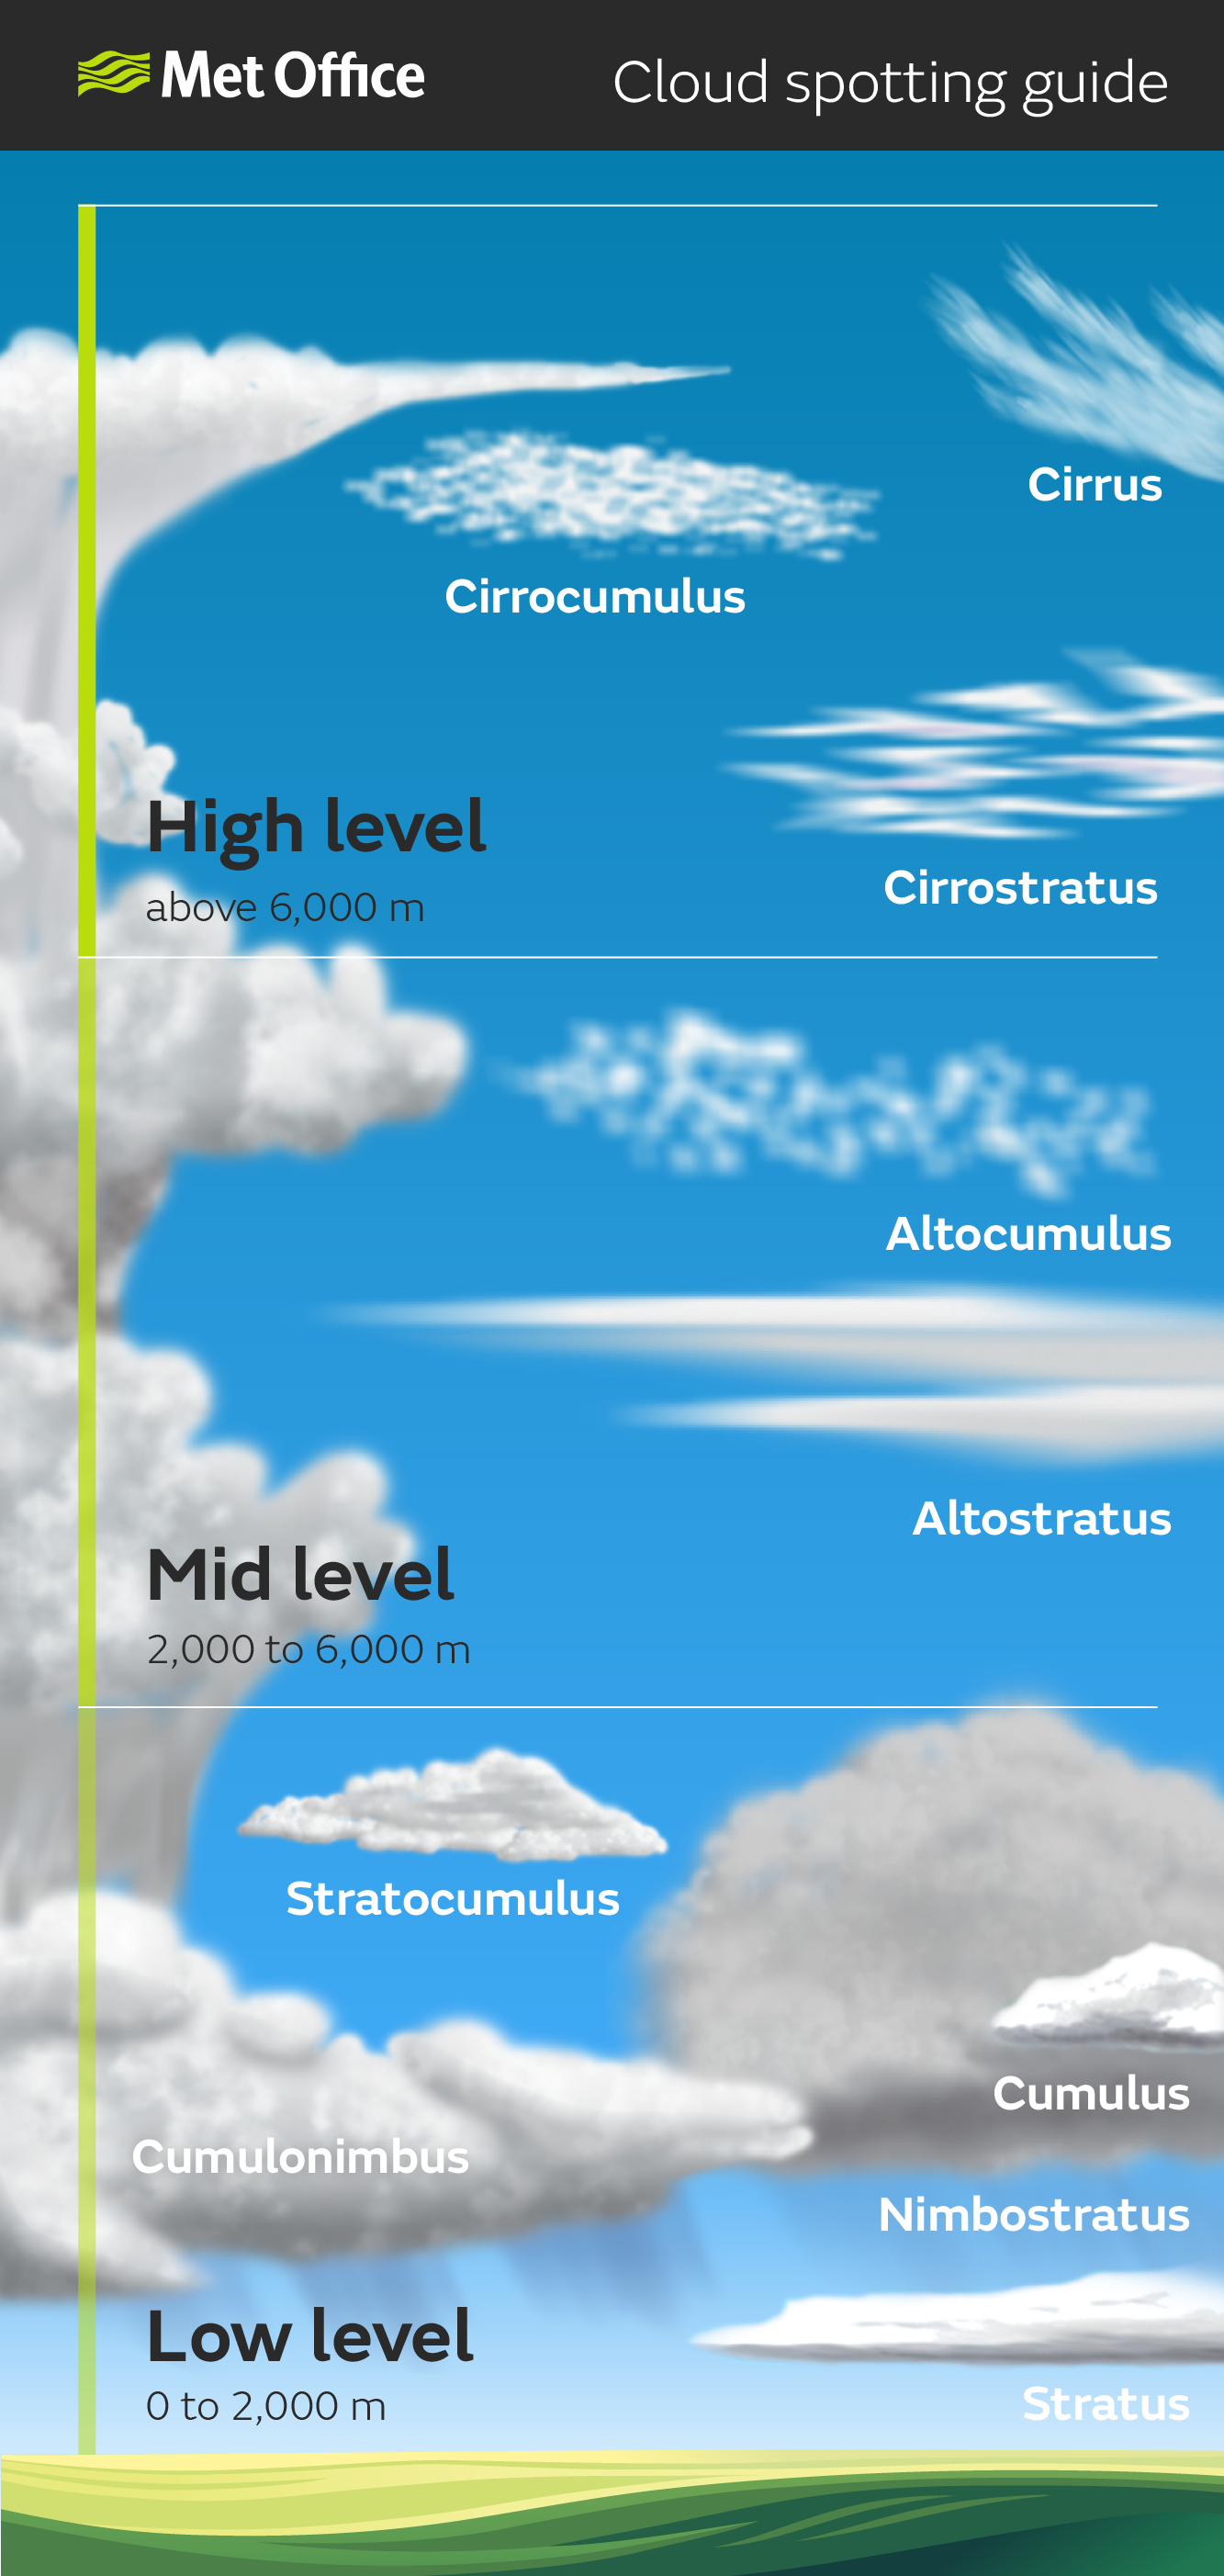
\includegraphics[height=10cm,keepaspectratio]{Cloud_infographic-01.png}
\caption{Schematische Darstellung der zehn Wolkengattungen}
    \label{fig:cloudtypes}
\end{figure}

Aufgrund der Ähnlichkeit einiger Klassen und der doch recht geringen Anzahl an Bildern im Vergleich zu der Anzahl an Klassen entschieden wir uns für eine Gruppierung in die vier Oberklassen \glqq Cirriform\grqq, \glqq Stratiform\grqq, \glqq Cumuliform\grqq, sowie \glqq Stratocumuliform\grqq, die in Tabelle \ref{table:oberklassen} beschrieben sind.

% TODO: Nochmal je ein typisches Bild pro Klasse aus unserem "echten" Datensatz????

\begin{table}[h!]
\begin{tabular}{l | p{3.5cm} | p{3.5cm} | l}
    Hauptklasse & Unterklassen & Beschreibung & \# Bilder \\ \hline
    Cirriform & Cirrus & gefedert, oft durchsichtig; sehr dünn und gefächert & 123 \\ \hline
    Stratiform & Cirrostratus, Altostratus, Nimbostratus, Stratus & sehr flächig, zusammenhängend; meist durchgängige Bedeckung & 129 \\ \hline
    Cumuliform & Cumulus, Cumulonimbus & große Haufen, \glqq Schäfchenwolken\grqq & 294 \\ \hline
    Stratocumuliform & Cirrocumulus, Altocumulus, Stratocumulus & viele kleine Haufen über eine große Fläche & 287 \\
\end{tabular}
    \caption{Zusammensetzung und Beschreibung unseres Klassifizierungsschemas}
    \label{table:oberklassen}
\end{table}
% TODO: evtl. Umwandlung der Tabelle in eigenständige "Abbildung"

Wie man auch schon an den Namen der verschiedenen Wolkengattungen sieht, gehen die Klassen leider teils ineinander über, was die Unterscheidung deutlich erschwert.
Außerdem gibt es noch sehr viele Arten, Unterarten und Begleitwolken, die sich teilweise ebenso in ihren Eigenschaften überschneiden.
Eine gute Übersicht der Wolkengattungen, -arten, etc. findet man in \cite{wiki:wolkenarten}.

\section{Methodik}
\label{sec:methodik}

% TODO: Methodik
%Hier sollte stehen, wie wir unser Problem lösen, sprich, wie unser Endsystem funktioniert.
%Warum machen wir es so und nicht anders?
%Wie funktionieren die Verfahren, die wir nutzen?
%Auch eine Ablaufgrafik wäre nice.

Im diesem Abschnitt erläutern wir die Methodik der beiden Klassifikationsansätze.
Eine Übersicht über den groben Ablauf kann in Abbildung \ref{fig:ablauf} gewonnen werden.
% TODO: Grafik baue ich noch ein, wobei ich nicht weiß, inwiefern ich da genau auf das neuronale Netz eingehen werde, die einzelnen Schichten zu zeigen wäre glaube ich leicht overkill.. --Max

\subsection{Vorverarbeitung der Bilder}

Da die Bilder verschieden waren, mussten wir sie vor der Klassifikation anpassen.
Zuerst haben wir unpassende Bilder, wie zum Beispiel von einem Sturm oder Fotos, auf denen die Wolken kaum erkennbar waren, manuell aussortiert.
Wie erwähnt war oft der untere Rand des Bildes nicht mehr nur reiner Himmel. Oft waren auch Wiesen oder Bäume zu sehen, die der Klassifizierung Probleme bereiteten.
Durch eine Binarisierung, die im Kapitel \ref{sec:binary} näher erläutert wird, konnten wir relativ akkurat den Himmel ausschneiden.
Zum Schluss haben wir die Bilder noch auf die einheitliche Größe von 500x500 Pixel gebracht, bei welcher die Algorithmen noch schnell ein genaues Ergebnis berechnen konnten.
Der Train/Validation-Split beim klassischen Ansatz war 8:2 bzw. 666:167.


\subsubsection{Binarisierung} 
\label{sec:binary}
Die Binarisierung haben wir mithilfe des arithmetischen Mittels über das gesamte Bild und dem Hue + Value aus dem HSV-Farbraum implementiert. % TODO: Wollen wir hier nicht eher die deutschen Begriffe verwenden? Hellwert, Farbwert, Sättigung und co?
Ein Pixel gehört dann zum Vordergrund, falls er heller ist als der Durchschnitt des gesamten Bildes, und falls er weder grün noch sehr sehr dunkel ist.
Dies hat nach vielem herum experimentieren für ein gutes Ergebnis gesorgt \ref{fig:boxAlg}.

\subsubsection{BoxCut Algrotithmus}
Nach dem Binarisieren wird von unten eine rechteckige Fläche des Bildes ausgewählt. Die Höhe beträgt dabei ca. 0.1 %oder lieber 10%?
des Bildes und die gesamte Breite (dargestellt durch das rote Rechteck im mittleren binarisierten Bild in \ref{fig:boxAlg}). In dem markierten Rechteck wird dann der durchschnittliche Farbwert berechnet, und falls dieser über unserem Treshhold%auch hier: lieber deutsch?
von 0.35 liegt, gehört ein Teil der Box wahrscheinlich zum Himmel, sodass das Bild bis zum unteren Teil der Box geschnitten wird.
Falls aber der durchschnittliche Farbwert unter dem Treshhold liegt, wird die Box um die Hälfte ihrer Höhe nach oben verschoben, bis letztlich der Treshhold überschritten wird.
%Hat der nächste Satz eigentlich eine Aussage :P? 
Wir haben mit vielen Bildern experimentiert, sodass wir unsere Werte angepasst haben, um beim Großteil auf ein gutes Ergebnis zu kommen.


\begin{figure}[h!]
\centering
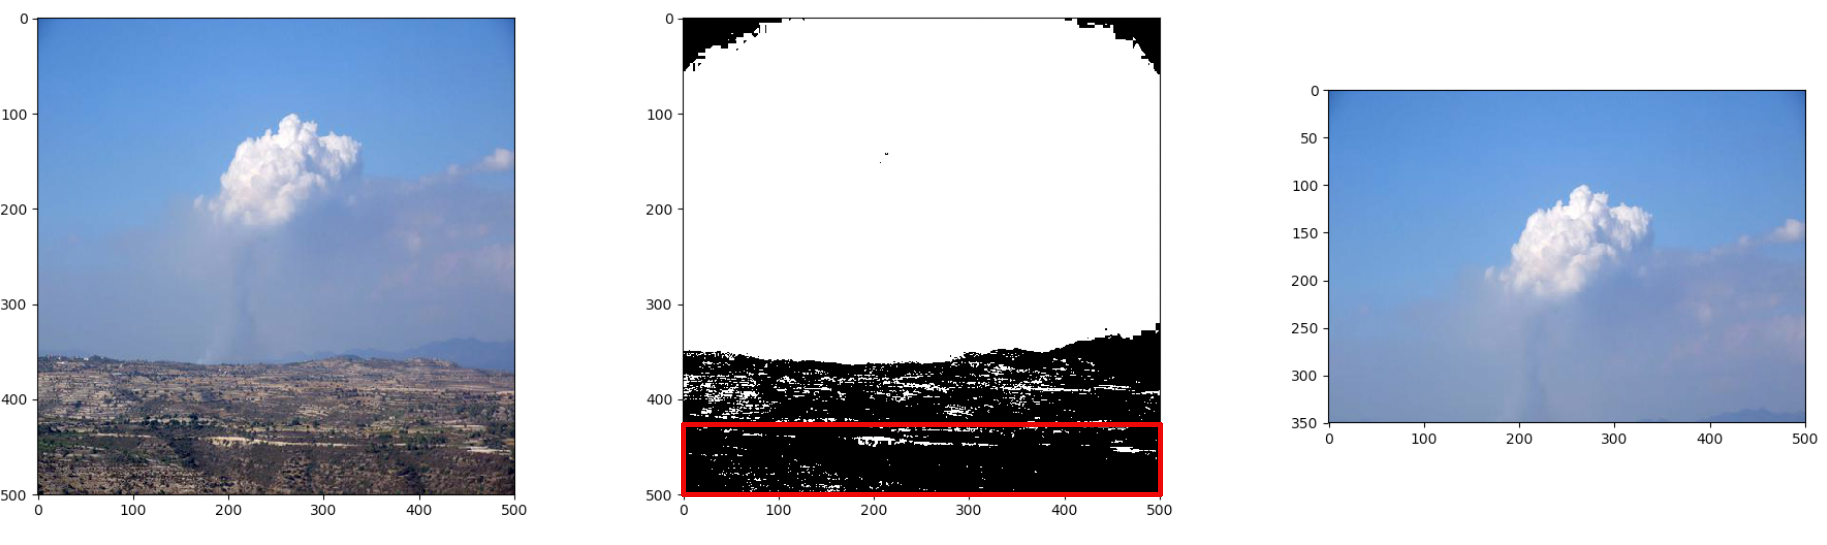
\includegraphics[width=1.1\textwidth]{boxAlg} %wäre schön das größer zu bekommen, ohne dass es sich verschiebt 
\caption{BoxCut-Algorithmus hat den Himmel erfolgreich von der Erde getrennt}
\label{fig:boxAlg}
\end{figure}

\subsubsection{Kantenzählung}
Ein Merkmal, welches wir neben dem Mittelwert, der Standardabweichung und den Farb-Histogrammen verwenden, misst die Anzahl der Kanten auf den Bildern.
Dazu wird zuerst das Bild in ein Graustufenbild umgewandelt, da man somit nicht die Kanten für jeden Farbwert im RGB-Farbraum einzeln berechnet werden müssen. Als nächstes wird ein Gaussfilter mit Sigma = 2 auf das Bild angewendet, damit nur die gröberen Kanten ins Gewicht fallen. Danach wird mit Hilfe des Sobel-Filters ein Kantenbild erzeugt.
Dort, wo sich Kanten befinden, sind die Pixel heller, d.h. die Werte sind höher.
Diese Werte werden dann zeilenweise aufsummiert, sodass ein Histogramm wie auf dem rechten Bild in Abbildung~\ref{fig:kaz} entsteht. So können die Kanten pro Zeile von zwei Bildern verglichen werden.

\begin{figure}[h!]
\centering
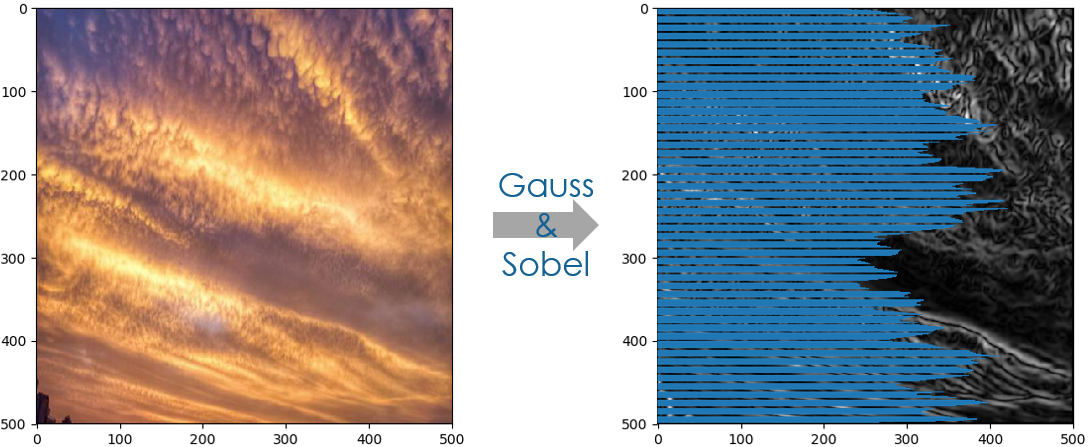
\includegraphics[width=\textwidth]{Kantenzaehlung.png}
\caption{Kantenzählung: Visualisierung der Funktion}
    \label{fig:kaz}
\end{figure}

\subsection{Augmentation der Bilder}
Da wir nur 800 Bilder zur Verfügung hatten, war es besonders für unser Convolutional Neural Network wichtig, mehr Bilder durch Augmentation zu erzeugen.
Hier haben wir uns dafür entschieden, dass nach dem Ausschneiden des Himmels%referenz auf die zugehörige Sektion ja/nein?
ein Bild jeweils in drei Teile geteilt wird wie in Abbildung \ref{fig:augmentation} zu erkennen.
Wichtig ist hierbei, dass dann die drei Bilder, die aus einem Bild entstanden sind, entweder alle in den Test- oder in den Validation-Split aufgenommen werden.

\begin{figure}[h!]
\centering
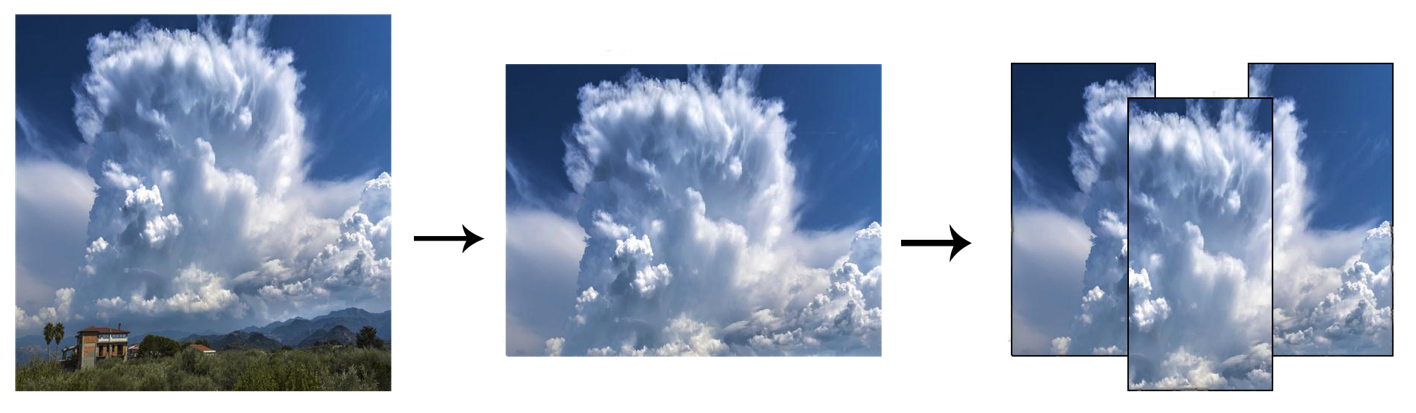
\includegraphics[width=\textwidth]{Augmentation}
\caption{Ein Bild wurde zu drei verschiedenen augmentiert}
    \label{fig:augmentation}
\end{figure}

\subsection{Gescheiterte Ansätze}
%Wollen wir diese section evtl under Experimente reinpacken? Hat ja schließlich nach experimentieren nicht ganz so gut funktioniert :P
Wir hatten noch zusätzliche Merkmale implementiert, die nicht gut genug funktioniert haben, um sie zu verwenden.
Ein Ansatz war es das Region Growing anzuwenden, um so aus den Bildern die Zusammenhangskomponenten der Wolken auszuscheiden oder auch um die Frequenzen der Regionen aus diesen abzuleiten.
Besonders bei der Klassifizierung von Cumuluswolken %"Schäfchenwolken"
wäre die Anzahl der Zusammenhangskomponenten sehr aussagekräftig gewesen.
Wir konnten das Region Growing leider nicht mit unseren Daten verwenden, da auf vielen Bildern die Wolken ineinander übergehen und trotz Runterskalierung auf 50p x 50p, die Berechnung pro Bild noch bis zu 30 Sekunden gedauert hat.


\section{Experimente und Ergebnisse}
\label{sec:experimente}
In diesem Abschnitt werden die erzielten Ergebnisse unter verschiedenen Parametern vorgestellt.

\subsection{Klassischer Ansatz}%TODO: Daten bei Änderungen aktualisieren
Die höchste Genauigkeit, die wir mit dem klassischen Ansatz erzielen konnten, beträgt 49\%. Wie gut dabei die einzelnen Merkmale abschneiden, kann man aus Tabelle~\ref{tab:gen} herauslesen. Dabei steht \textit{mean} für den Mittelwert und \textit{std} für die Standardabweichung. 
%Was bedeutet der "grau" Eintrag in der ersten Tabelle?
\begin{table}[h]
\begin{tabular}{|l|l|l|l|l|l|l|}
 \hline
 \textbf{Merkmale:}&mean&std&1D-Hist.&3D-Hist.&Grau-Hist.&Kantenz.\\
 \hline
 \textbf{Erfolg:} & 28\% & 32\% & 35\% & 38\% & grau & 41\% \\
 \hline
\end{tabular}
\caption{Genauigkeit der einzelnen Merkmale, gerundet}
\label{tab:gen}
\end{table}

\begin{table}[h]
\begin{tabular}{|l|l|l|l|}
 \hline
 \textbf{Kombi.:}&mean+std&mean+std+Kantenz.&Kantenz.+3D-Hist.\\
 \hline
 \textbf{Erfolg:} & 40\% & 48\% & 49\% \\
 \hline
\end{tabular}
\caption{Genauigkeit von Merkmalskombinationen, gerundet}
\label{tab:gen2}
\end{table}

Abbildung~\ref{fig:meanstd} zeigt, dass die verschiedenen Klassen mithilfe von Mittelwert und Standardabweichung nur schwer auseinanderzuhalten sind und sich nicht leicht in verschiedene Klassen trennen lassen. Trotzdem erreichen wir hier nur mit diesen beiden Merkmalen eine Genauigkeit von 40\%.
\begin{figure}[h!]
\hspace*{-3cm}
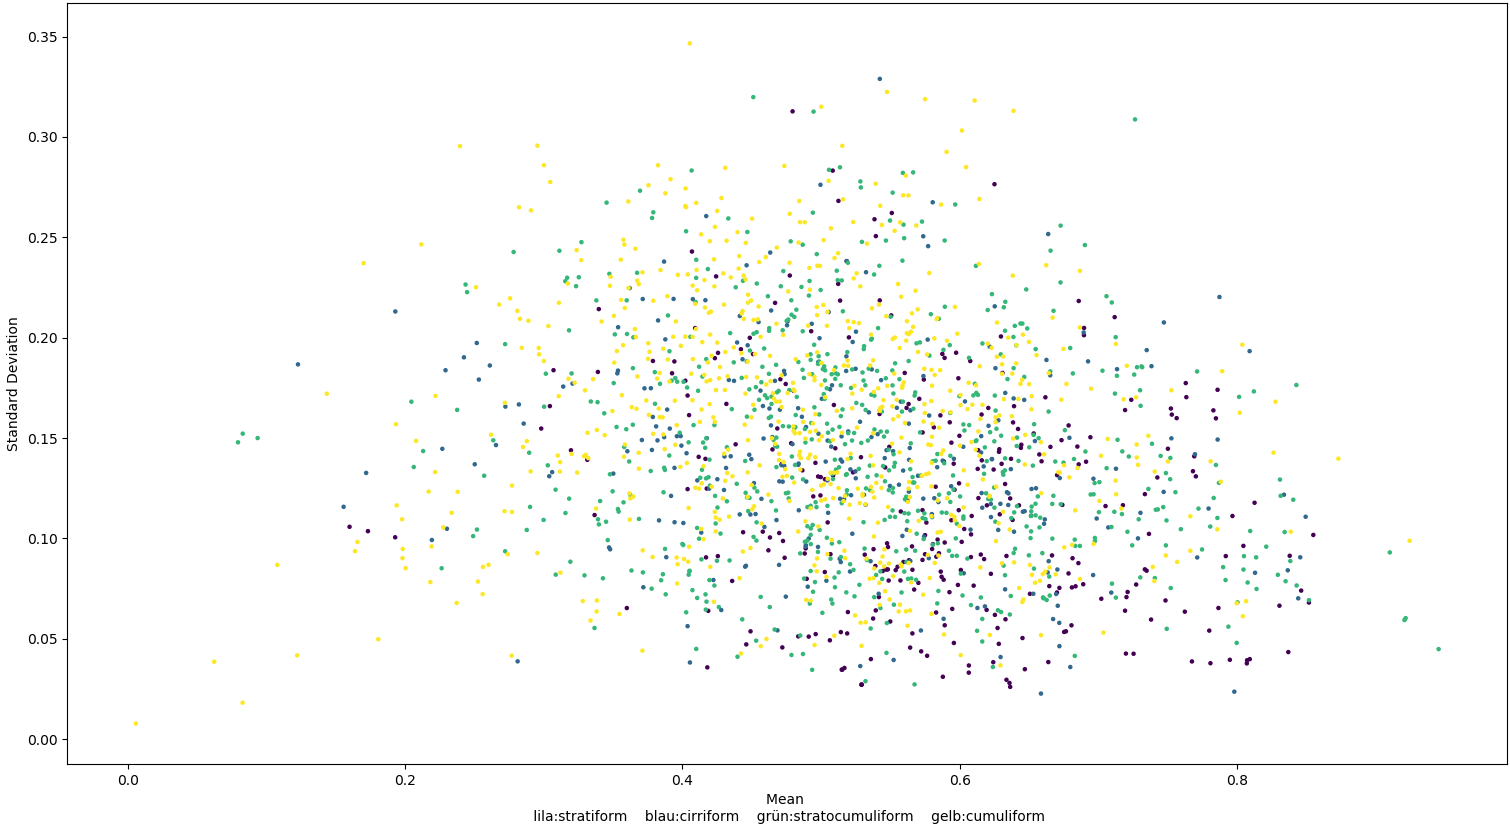
\includegraphics[width=1.5\textwidth]{Scatterplot_mean_std.png}
\caption{Scatterplot für Mittelwert und Standardabweichung}
\label{fig:meanstd}
\end{figure}

Bei der Kantenzählung wurden beim Gaussschen Weichzeichner verschiedene Sigma Werte ausprobiert, wobei sich Sigma = 2 als am besten herausstellte (siehe Tabelle~\ref{tab:sigma}).
Dies ist so, da bei größeren Sigmas die Kanten zu sehr verschwimmen %<-- Bin mir da nicht 100% sicher, ob das stimmt, weil ich nicht weiß, ob ich Sigma richtig verstanden habe... || so hätte ich das auch verstanden - Max
\begin{table}[h]
\begin{tabular}{|l|l|l|l|l|l|}
 \hline
 \textbf{Sigma:} & 0 & 1 & 2 & 3 & 4\\
 \hline
 \textbf{Erfolg:} & 40\% & 41\% & 41\% & 36\% & 35\% \\
 \hline
\end{tabular}
\caption{Genauigkeit der Kantenzählung bei verschiedenen Sigmas für den Weichzeichner}
\label{tab:sigma}
\end{table}

Die Kantenzählung war besonders darauf ausgelegt, stratiforme Wolken %(flächige Wolken)
zu identifizieren, da diese meist durchgängige Flächen sind und daher wenig Kanten haben.
Abbildung~\ref{fig:kbs} zeigt einen Boxplot und einen Swarmplot für die Kantenzählung.
Dabei ist wichtig zu berücksichtigen, dass für die Plots die Histogramme auf einen Wert reduziert wurden, das heißt der Plot spiegelt das Merkmal nur annäherungsweise wieder.
Während der Boxplot vermuten lässt, die stratiformen Wolken ließen sich mithilfe des Merkmals alleine klar von den anderen trennen, zeigt der Swarmplot, dass dies nur für etwa die Hälfte der Bilder mit stratiformen Wolken gilt. %Also haben wir das Merkmal so für unseren Entscheidungsbaum verwendet, dass wir alle Wolken die einen Gesamtkantenwert von unter 1000 haben als stratiform klassifizieren, dabei aber nicht ausschließen, dass unter den Verbliebenen noch stratiforme Wolken sind...könnte man hier schreiben wenn wir es machen.

\begin{figure}[h!]%Die Bilder sind eventuell zu klein, dann bitte einfach untereinander statt nebeneinander.
\subfigure[Boxplot Kantenzählung]
{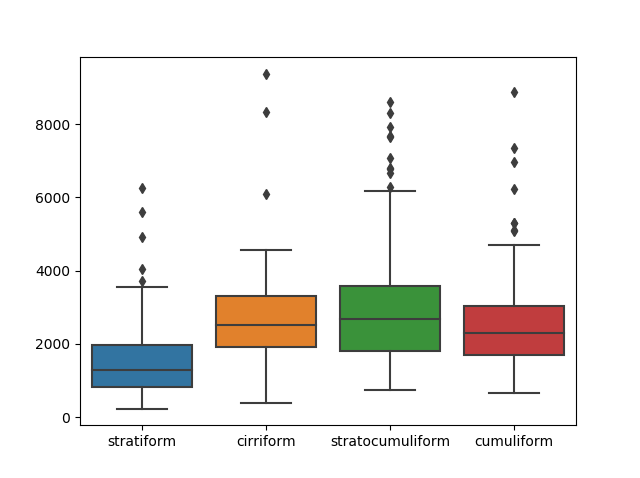
\includegraphics[width=0.53\textwidth]{edge_count_boxplot.png}}
\subfigure[Swarmplot Kantenzählung]
{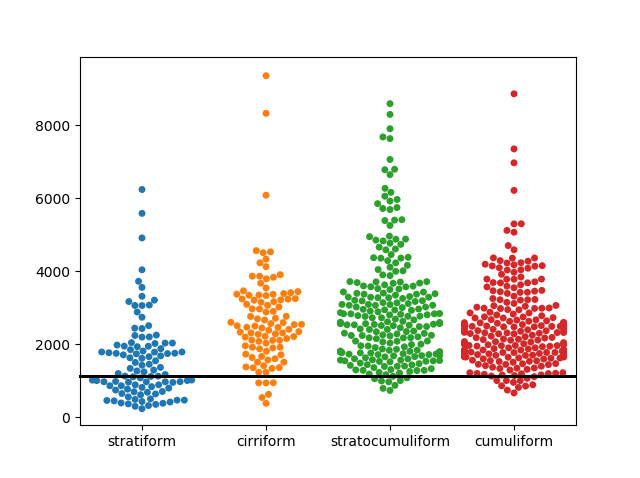
\includegraphics[width=0.53\textwidth]{edge_count_swarmplot.png}}
\caption{Kantenzählung: Unterschiede der Klassen}
    \label{fig:kbs}
\end{figure}

\subsection{Neuronale Netze}
% TODO: Fazit
%Wie sehen unsere Ergebnisse aus?
%Wie verändern sich die Ergebnisse durch die CNNs?
%Was passiert, wenn man einzelne Teile des Systems austauscht oder Merkmale entfernt (dies evtl.\ auch mit Diagrammen zeigen)?
%Wie schneidet das System pro Klasse ab?
%Wie wirken sich Änderungen der Parameter/Hyperpara\-meter auf die Ergebnisse aus?
%Wie schnell sind unsere Verfahren?

\subsection{Menschen klassifizieren Wolken}

Da uns aufgefallen ist, dass es nicht nur für den Computer sondern auch für uns schwierig ist, die Wolken zu klassifizieren, haben wir uns dazu entschieden, eine kleine Studie durchzuführen.
Bei dieser Studie sollten die sechs getesteten Probanden jeweils sechzehn Wolkenbilder in unsere vier Kategorien einteilen.
Sie haben die Übersicht aus Abbildung~\ref{fig:cloudtypes} bekommen und pro Klasse sechs Trainingsbilder als Referenz.
Dabei wurde eine Durchschnittliche Genauigkeit von 51\% erreicht. Der Versuchsaufbau und die Ergebnisse sind noch einmal genauer in Anhang 1 %oder der wievielte Anhang auch immer.. bitte aktualisieren/korrigieren
geschildert.

% TODO: Zumindest oberflächlicher Vergleich der verschiedenen Ansätze und der Menschen.

\section{Fazit}
\label{sec:fazit}

% TODO: Fazit
%Was ist unser Fazit?
%Zusammenfassung und Einordnung unserer Ergebnisse.
%Ausblick?

Insgesamt können wir sagen, dass es eine Herausforderung war, die verschiedenen Bilder zu klassifizieren.
Nicht nur innerhalb einer Wolkenart unterscheiden sich die Bilder teils sehr stark voneinander, auch ist es vor allem die Ähnlichkeit vieler Bilder in jeweils verschiedenen Wolkenklassen, die die korrekte Klassifizierung der Wolken erschwert.
Und da es sogar für Menschen schwer ist, viele Bilder ihrer richtigen Kategorie zuzuordnen, hatten wir besonders bei der klassischen Methode nicht all zu genaue Ergebnisse erwartet.
Allerdings sind wir mit 49\% für die klassische Methodik schon sehr zufrieden, da dies noch weit besser ist, als ein zufälliges Zuordnen der Klassen.

Beim Neuronale Netze .... % TODO

Wir könnten uns vorstellen, dass ein viel besseres Ergebnis zu erreichen ist, wenn die Bilder alle nach einer bestimmten Norm aufgenommen wären, zum Beispiel mit dem selben Winkel zum Himmel, bei gleicher Helligkeit oder aber vom selben Standpunkt aus.
Allerdings müsste man dann äußerst vorsichtig sein, wie im Falle der Kieler Universität, das die Bilder so nicht zum overfitten der Ergebnisse führen.%Sollte das evtl in die Bibliografie hinein?

\bibliographystyle{babplain}
\bibliography{bibliography}

\end{document}
